
\documentclass[handout]{beamer}
\usetheme{Singapore}
\usecolortheme[RGB={0, 32, 91}]{structure}  % Rice blue
\setbeamertemplate{navigation symbols}{\insertframenumber}

\usepackage{tcolorbox}
\usepackage{tikz}
\usetikzlibrary{decorations.pathmorphing}

\definecolor{riceblue}{rgb}{0.000, 0.125, 0.357}
\definecolor{ricegray}{rgb}{0.486, 0.494, 0.498}
\definecolor{ricerichblue}{rgb}{0.039, 0.314, 0.620}

\title{Estimating individual contributions to \\ team success in women's college volleyball}
\author{\color{ricerichblue} Scott Powers, Luke Stancil and Naomi Consiglio}
\date{NESSIS 2023}

\begin{document}

\begin{frame}[noframenumbering]
  \maketitle
  \vfill
  \hfill\includegraphics[width = 4cm]{images/rice_logo.png}
\end{frame}

\begin{frame}{Outline}
  \centering
  {\color{riceblue} \bf Act 1: Estimating Point Win Probability}\\
  {\color{ricegray} \it Technique: Markov Chain Model}\\
  ~\\
  {\color{riceblue} \bf Act 2: Evaluating Individual Contributions}\\
  {\color{ricegray} \it Technique: Domain Knowledge}\\
  ~\\
  {\color{riceblue} \bf Act 3: Adjusting for Strength of Schedule}\\
  {\color{ricegray} \it Technique: Linear Mixed-Effect Models}
\end{frame}

\begin{frame}
  \centering
  \color{riceblue} \bf (Act 0: Introduction to Volleyball)\\
\end{frame}

\begin{frame}{Introduction to Volleyball}
  \begin{columns}
    \begin{column}{0.4\textwidth}
      \centering
      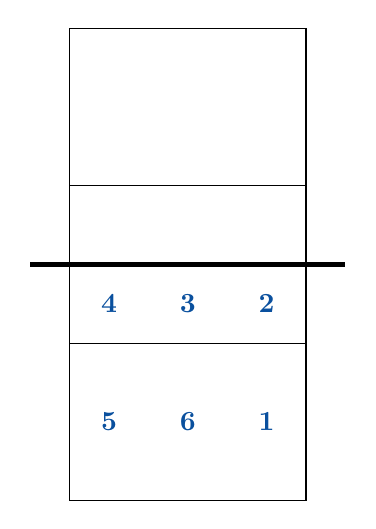
\begin{tikzpicture}
        \draw[line width = 2pt] (-0.5, 3) -- (3.5, 3);
        \draw (0, 0) -- (0, 6);
        \draw (3, 0) -- (3, 6);
        \draw (0, 0) -- (3, 0);
        \draw (0, 2) -- (3, 2);
        \draw (0, 4) -- (3, 4);
        \draw (0, 6) -- (3, 6);
        \node (1) at (2.5, 1) {\bf\color{ricerichblue} 1};
        \node (2) at (2.5, 2.5) {\bf\color{ricerichblue} 2};
        \node (3) at (1.5, 2.5) {\bf\color{ricerichblue} 3};
        \node (4) at (0.5, 2.5) {\bf\color{ricerichblue} 4};
        \node (5) at (0.5, 1) {\bf\color{ricerichblue} 5};
        \node (6) at (1.5, 1) {\bf\color{ricerichblue} 6};
      \end{tikzpicture}
    \end{column}
    \begin{column}{0.6\textwidth}
    \end{column}
  \end{columns}
\end{frame}

\begin{frame}[noframenumbering]{Introduction to Volleyball}
  \begin{columns}
    \begin{column}{0.4\textwidth}
      \centering
      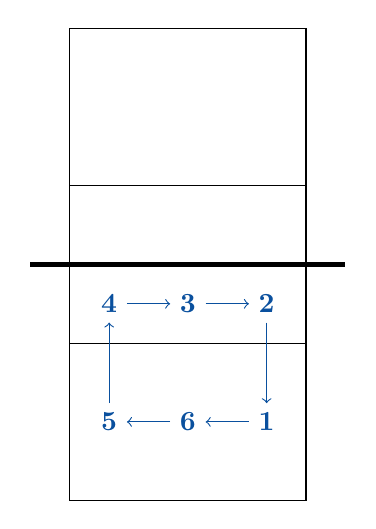
\begin{tikzpicture}
        \draw[line width = 2pt] (-0.5, 3) -- (3.5, 3);
        \draw (0, 0) -- (0, 6);
        \draw (3, 0) -- (3, 6);
        \draw (0, 0) -- (3, 0);
        \draw (0, 2) -- (3, 2);
        \draw (0, 4) -- (3, 4);
        \draw (0, 6) -- (3, 6);
        \node (1) at (2.5, 1) {\bf\color{ricerichblue} 1};
        \node (2) at (2.5, 2.5) {\bf\color{ricerichblue} 2};
        \node (3) at (1.5, 2.5) {\bf\color{ricerichblue} 3};
        \node (4) at (0.5, 2.5) {\bf\color{ricerichblue} 4};
        \node (5) at (0.5, 1) {\bf\color{ricerichblue} 5};
        \node (6) at (1.5, 1) {\bf\color{ricerichblue} 6};
        \draw[->, color = ricerichblue] (1) -- (6);
        \draw[->, color = ricerichblue] (6) -- (5);
        \draw[->, color = ricerichblue] (5) -- (4);
        \draw[->, color = ricerichblue] (4) -- (3);
        \draw[->, color = ricerichblue] (3) -- (2);
        \draw[->, color = ricerichblue] (2) -- (1);
      \end{tikzpicture}
    \end{column}
    \begin{column}{0.6\textwidth}
    \end{column}
  \end{columns}
\end{frame}

\begin{frame}{Introduction to Volleyball}
  \begin{columns}
    \begin{column}{0.4\textwidth}
      \centering
      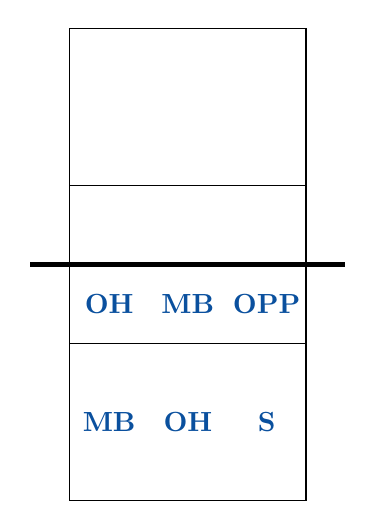
\begin{tikzpicture}
        \draw[line width = 2pt] (-0.5, 3) -- (3.5, 3);
        \draw (0, 0) -- (0, 6);
        \draw (3, 0) -- (3, 6);
        \draw (0, 0) -- (3, 0);
        \draw (0, 2) -- (3, 2);
        \draw (0, 4) -- (3, 4);
        \draw (0, 6) -- (3, 6);
        \node (1) at (2.5, 1) {\bf\color{ricerichblue} S};
        \node (2) at (2.5, 2.5) {\bf\color{ricerichblue} OPP};
        \node (3) at (1.5, 2.5) {\bf\color{ricerichblue} MB};
        \node (4) at (0.5, 2.5) {\bf\color{ricerichblue} OH};
        \node (5) at (0.5, 1) {\bf\color{ricerichblue} MB};
        \node (6) at (1.5, 1) {\bf\color{ricerichblue} OH};
     \end{tikzpicture}
    \end{column}
    \begin{column}{0.6\textwidth}
      \small
      \color{ricerichblue}\bf Setter (S)\\
      \color{black}\it Setting\\
      ~\\
      \color{ricerichblue}\bf Outside Hitter (OH)\\
      \color{black}\it Attacking, Passing\\
      ~\\
      \color{ricerichblue}\bf Middle Blocker (MB)\\
      \color{black}\it Blocking, Attacking\\
      ~\\
      \color{ricerichblue}\bf Opposite Hitter (OPP)\\
      \color{black}\it Attacking, Blocking\\
      ~\\
      \color{white}\bf Libero (L)\\
      \color{white}\it Passing
    \end{column}
  \end{columns}
\end{frame}

\begin{frame}[noframenumbering]{Introduction to Volleyball}
  \begin{columns}
    \begin{column}{0.4\textwidth}
      \centering
      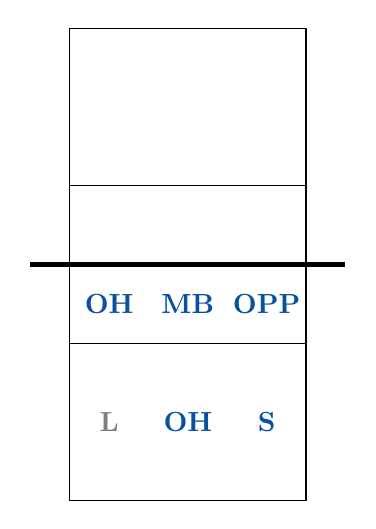
\begin{tikzpicture}
        \draw[line width = 2pt] (-0.5, 3) -- (3.5, 3);
        \draw (0, 0) -- (0, 6);
        \draw (3, 0) -- (3, 6);
        \draw (0, 0) -- (3, 0);
        \draw (0, 2) -- (3, 2);
        \draw (0, 4) -- (3, 4);
        \draw (0, 6) -- (3, 6);
        \node (1) at (2.5, 1) {\bf\color{ricerichblue} S};
        \node (2) at (2.5, 2.5) {\bf\color{ricerichblue} OPP};
        \node (3) at (1.5, 2.5) {\bf\color{ricerichblue} MB};
        \node (4) at (0.5, 2.5) {\bf\color{ricerichblue} OH};
        \node (5) at (0.5, 1) {\bf\color{ricegray} L};
        \node (6) at (1.5, 1) {\bf\color{ricerichblue} OH};
      \end{tikzpicture}
    \end{column}
    \begin{column}{0.6\textwidth}
      \small
      \color{ricerichblue}\bf Setter (S)\\
      \color{black}\it Setting\\
      ~\\
      \color{ricerichblue}\bf Outside Hitter (OH)\\
      \color{black}\it Passing, Attacking\\
      ~\\
      \color{ricerichblue}\bf Middle Blocker (MB)\\
      \color{black}\it Blocking, Attacking\\
      ~\\
      \color{ricerichblue}\bf Opposite Hitter (OPP)\\
      \color{black}\it Blocking, Attacking\\
      ~\\
      \color{ricegray}\bf Libero (L)\\
      \color{black}\it Passing
    \end{column}
  \end{columns}
\end{frame}

\begin{frame}{Existing metrics}
  \begin{itemize}
    \item Standard metrics
    \begin{itemize}
      \item Serving: Ace\%, Error\%
      \item Receiving: Error\%, Passer Rating
      \item Digging: Digs / Set, Digs / Opportunity
      \item Setting: Assists / Set
      \item Attacking: Hitting Efficiency = (Kills -- Errors) / Attempts
      \item Blocking: Blocks / Set
    \end{itemize}
    ~\\
    \item State of the art
    \begin{itemize}
      \item Fellingham (JQAS 2022): PAAPS
      \begin{itemize}
        \item Similar to regularized adjusted plus-minus in basketball
      \end{itemize}
      \item Gordon (volleydork.com): Value Added above Expectation
      \begin{itemize}
        \item Very similar to the present work
      \end{itemize}
    \end{itemize}
  \end{itemize}
\end{frame}

\begin{frame}
  \centering
  {\color{riceblue} \bf Act 1: Estimating Point Win Probability}\\
  {\color{ricegray} \it Technique: Markov Chain Model}
\end{frame}

\begin{frame}{{\it Example:} First Point of 2022 National Championship}{\bf \color{orange} Texas \color{red} Louisville}
  \begin{center}
    \small
    \begin{tabular}{llccc}
      \bf Player                      & \bf Skill                 & \bf Eval          & \bf (X, Y)                  & \bf Attack Code\\
      \hline
      \color{red} Anna Deeber         & \color{red} Serve         & \color{red} --    & \color{red} (2.99, -0.13)\\
      \color{orange} Emma Halter      & \color{orange} Reception  & \color{orange} \# & \color{orange} (0.93, 5.80)\\
      \color{orange} Saige K.-Torres  & \color{orange} Set        & \color{orange} \# & \color{orange} (2.13, 3.13)\\
      \color{orange} Molly Phillips   & \color{orange} Attack     & \color{orange} -- & \color{orange} (3.33, 3.20) & \color{orange} X6\\
      \color{red} Raquel Lazaro       & \color{red} Dig           & \color{red} +     & \color{red} (0.86, 4.98)\\
      \color{red} Elena Scott         & \color{red} Set           & \color{red} \#    & \color{red} (2.99, 1.65)\\
      \color{red} Claire Chaussee     & \color{red} Attack        & \color{red} --    & \color{red} (0.63, 2.83)    & \color{red} V5\\
      \color{orange} Kayla Caffey     & \color{orange} Block      & \color{orange} +  & \color{orange} (3.26, 3.43)\\
      \color{red} Phekran Kong        & \color{red} Dig           & \color{red} !     & \color{red} (0.89, 3.13)\\
      \color{red} Raquel Lazaro       & \color{red} Set           & \color{red} \#    & \color{red} (0.97, 2.61)\\
      \color{red} Claire Chaussee     & \color{red} Attack        & \color{red} \#    & \color{red} (0.67, 2.91)    & \color{red} X5
    \end{tabular}
  \end{center}
  \small
  Evaluation Codes: {\bf \# $>$ + $>$ ! $>$ -- $>$ / $>$ =}\\
  Dataset: 4,147 matches, 600K+ points, 5M+ contacts, $\sim$6,000 players
\end{frame}

\begin{frame}{Markov Chain Model: Game State}
  \begin{tcolorbox}
    {\it Definition:} A {\bf volley} is a sequence of consecutive contacts by the same team
  \end{tcolorbox}
  ~\\
  The game state on each contact is given by:
  \begin{itemize}
    \item Whether the team started the point by serving or receiving
    \item The sequence of contacts made during the current volley\\
      (including evaluation code {\it except} for contacts ending a volley)
  \end{itemize}
  ~\\
  Terminal states: (S, P) and (R, P)\\
  ~\\
  {\it Example:} (S, D\#) $\rightarrow$ (S, D\#S\#) $\rightarrow$ (S, D\#S\#A) $\rightarrow$ (R, P)\\
\end{frame}

\begin{frame}{{\it Example:} First Point of 2022 National Championship}
  \centering
  \begin{tabular}{llc|cc}
    \bf Player                      & \bf Skill                 & \bf Eval            & \bf State                   & \bf P(Sideout)\\
    \hline
    \color{red} Anna Deeber         & \color{red} Serve         &                     & \color{red} (S, SV)         & \color{orange} 57\%\\
    \color{orange} Emma Halter      & \color{orange} Reception  & \color{orange} \#   & \color{orange} (R, R\#)     & \color{orange} 63\%\\
    \color{orange} Saige K.-Torres  & \color{orange} Set        & \color{orange} \#   & \color{orange} (R, R\#S\#)  & \color{orange} 64\%\\
    \color{orange} Molly Phillips   & \color{orange} Attack     &                     & \color{orange} (R, R\#S\#A) & \color{orange} 64\%\\
    \color{red} Raquel Lazaro       & \color{red} Dig           & \color{red} +       & \color{red} (S, D+)         & \color{orange} 49\%\\
    \color{red} Elena Scott         & \color{red} Set           & \color{red} \#      & \color{red} (S, D+S\#)      & \color{orange} 47\%\\
    \color{red} Claire Chaussee     & \color{red} Attack        &                     & \color{red} (S, D+S\#A)     & \color{orange} 47\%\\
    \color{orange} Kayla Caffey     & \color{orange} Block      & \color{orange} +    & \color{orange} (R, B+)      & \color{orange} 56\%\\
    \color{red} Phekran Kong        & \color{red} Dig           & \color{red} !       & \color{red} (S, D!)         & \color{orange} 51\%\\
    \color{red} Raquel Lazaro       & \color{red} Set           & \color{red} \#      & \color{red} (S, D!S\#)      & \color{orange} 51\%\\
    \color{red} Claire Chaussee     & \color{red} Attack        &                     & \color{red} (S, D!S\#A)     & \color{orange} 51\%\\
    \hline
    \bf\color{red} Point Louisville &                           &                     &                             & \color{orange} \bf 0\%\\
  \end{tabular}
\end{frame}

\begin{frame}
  \centering
  {\color{riceblue} \bf Act 2: Evaluating Individual Contributions}\\
  {\color{ricegray} \it Technique: Domain Knowledge}
\end{frame}

\begin{frame}{How a Point Progresses}
  \centering
  \begin{tabular}{l|l|l|l|l}
    \bf Volley 1  & \bf Volley 2  & \bf Volley 3  & \bf Volley 4  & \bf Volley 5\\
    \bf Team A    & \bf Team B    & \bf Team A    & \bf Team B    & \bf Team A\\
    \hline
    Serve         &               &               &               &\\
                  & Reception     &               &               &\\
                  & Set           &               &               &\\
                  & Attack        &               &               &\\
                  &               & Dig           &               &\\
                  &               & Set           &               &\\
                  &               & Attack        &               &\\
                  &               &               & Dig           &\\
                  &               &               & Set           &\\
                  &               &               & Attack        &\\
                  &               &               &               & Dig\\
                  &               &               &               & ...
  \end{tabular}
\end{frame}

\begin{frame}{How a Point Progresses}
  \centering
  \begin{tabular}{lllll}
    \bf Volley 1  & \bf Volley 2  & \bf Volley 3  & \bf Volley 4  & \bf Volley 5\\
    \bf Team A    & \bf Team B    & \bf Team A    & \bf Team B    & \bf Team A\\
    \hline
    \cline{1-2}
    \multicolumn{1}{|l}{Serve}  & \multicolumn{1}{l|}{Reception}\\
    \cline{1-2}
                                & Set\\
    \cline{2-3}
                                & \multicolumn{1}{|l}{Attack} & \multicolumn{1}{l|}{Dig}\\
    \cline{2-3}
                                &                             & Set\\
    \cline{3-4}
                                &                             & \multicolumn{1}{|l}{Attack} & \multicolumn{1}{l|}{Dig}\\
    \cline{3-4}
                                &                             &                             & Set\\
    \cline{4-5}
                                &                             &                             & \multicolumn{1}{|l}{Attack} & \multicolumn{1}{l|}{Dig}\\
    \cline{4-5}
                                &                             &                             &                             & ...
  \end{tabular}
\end{frame}

\begin{frame}[noframenumbering]{How a Point Progresses}
  \centering
  \begin{tabular}{lllll}
    \bf Volley 1  & \bf Volley 2  & \bf Volley 3  & \bf Volley 4  & \bf Volley 5\\
    \bf Team A    & \bf Team B    & \bf Team A    & \bf Team B    & \bf Team A\\
    \hline
    \cline{1-2}
    \multicolumn{1}{|l}{Serve}  & \multicolumn{1}{l|}{Reception}\\
    \cline{1-2}
    \cline{2-3}
                                & \multicolumn{1}{|l}{Set}    & \multicolumn{1}{l|}{}\\
                                & \multicolumn{1}{|l}{Attack} & \multicolumn{1}{l|}{Dig}\\
    \cline{2-3}
    \cline{3-4}
                                &                             & \multicolumn{1}{|l}{Set}    & \multicolumn{1}{l|}{}\\
                                &                             & \multicolumn{1}{|l}{Attack} & \multicolumn{1}{l|}{Dig}\\
    \cline{3-4}
    \cline{4-5}
                                &                             &                             & \multicolumn{1}{|l}{Set}    & \multicolumn{1}{l|}{}\\
                                &                             &                             & \multicolumn{1}{|l}{Attack} & \multicolumn{1}{l|}{Dig}\\
    \cline{4-5}
                                &                             &                             &                             & ...
  \end{tabular}
\end{frame}

\begin{frame}{Attack Outcome Tree}
  \centering
  \begin{tikzpicture}
    \node (Attack) at (0, 0) {\small Attack};
    \node (Attack Error) at (-1.5, -1.2) {\small Error};
    \node (Attack No Error) at (1.5, -1.2) {\small No};
    \node (Block) at (0, -2.4) {\small Block};
    \node (No Block) at (3, -2.4) {\small No};
    \node (Block No Error) at (-1.5, -3.6) {\small No};
    \node (Block Error) at (1.5, -3.6) {\small Error};
    \node (Return) at (-3, -4.8) {\small Return};
    \node (Through) at (0, -4.8) {\small Through};
    \node (No Block Dig/Kill) at (4.5, -3.6) {\small Dig/Kill};
    \node (Return Dig/Kill) at (-3, -6) {\small Dig/Kill};
    \node (Through Dig/Kill) at (0, -6) {\small Dig/Kill};
    \draw[->] (Attack) -- (Attack Error);
    \draw[->] (Attack) -- (Attack No Error);
    \draw[->] (Attack No Error) -- (Block);
    \draw[->] (Attack No Error) -- (No Block);
    \draw[->] (Block) -- (Block No Error);
    \draw[->] (Block) -- (Block Error);
    \draw[->] (Block No Error) -- (Return);
    \draw[->] (Block No Error) -- (Through);
    \draw[->, decorate, decoration = snake] (No Block) -- (No Block Dig/Kill);
    \draw[->, decorate, decoration = snake] (Return) -- (Return Dig/Kill);
    \draw[->, decorate, decoration = snake] (Through) -- (Through Dig/Kill);
    \node at (0, -0.9) {\tiny \color{white} 91\% ATT; 9\% SET};
    \node at (1.5, -1.8) {\tiny \color{white} 100\% BLK};
    \node at (1.5, -2.1) {\tiny \color{white} 70\% ATT; 30\% SET};
    \node at (0, -3) {\tiny \color{white} 100\% BLK};
    \node at (0, -3.3) {\tiny \color{white} 81\% ATT; 19\% SET};
    \node at (-1.5, -4.2) {\tiny \color{white} 100\% BLK};
    \node at (-1.5, -4.5) {\tiny \color{white} 73\% ATT; 27\% SET};
    \node at (1.2, -5.2) {\tiny \color{white} 28\% BLK; 72\% DIG};
    \node at (1.2, -5.5) {\tiny \color{white} 79\% ATT; 21\% SET};
    \node at (-3.75, -5.2) {\tiny \color{white} 100\% BLK};
    \node at (-4.2, -5.5) {\tiny \color{white} 89\% ATT; 11\% SET};
    \node at (5, -2.6) {\tiny \color{white} 52\% BLK; 48\% DIG};
    \node at (5, -2.9) {\tiny \color{white} 69\% ATT; 31\% SET};
  \end{tikzpicture}
\end{frame}

\begin{frame}[noframenumbering]{Attack Outcome Tree}
  \centering
  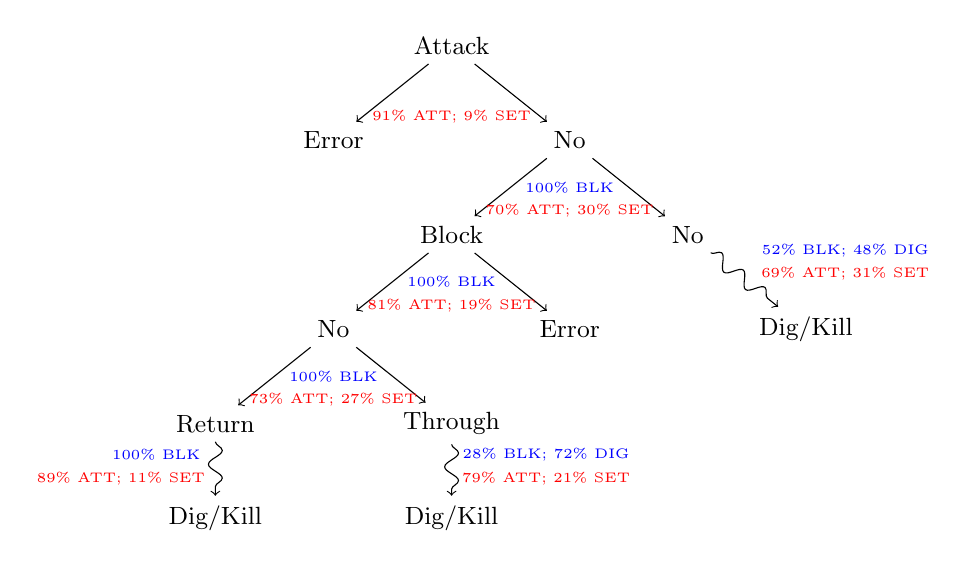
\begin{tikzpicture}
    \node (Attack) at (0, 0) {\small Attack};
    \node (Attack Error) at (-1.5, -1.2) {\small Error};
    \node (Attack No Error) at (1.5, -1.2) {\small No};
    \node (Block) at (0, -2.4) {\small Block};
    \node (No Block) at (3, -2.4) {\small No};
    \node (Block No Error) at (-1.5, -3.6) {\small No};
    \node (Block Error) at (1.5, -3.6) {\small Error};
    \node (Return) at (-3, -4.8) {\small Return};
    \node (Through) at (0, -4.8) {\small Through};
    \node (No Block Dig/Kill) at (4.5, -3.6) {\small Dig/Kill};
    \node (Return Dig/Kill) at (-3, -6) {\small Dig/Kill};
    \node (Through Dig/Kill) at (0, -6) {\small Dig/Kill};
    \draw[->] (Attack) -- (Attack Error);
    \draw[->] (Attack) -- (Attack No Error);
    \draw[->] (Attack No Error) -- (Block);
    \draw[->] (Attack No Error) -- (No Block);
    \draw[->] (Block) -- (Block No Error);
    \draw[->] (Block) -- (Block Error);
    \draw[->] (Block No Error) -- (Return);
    \draw[->] (Block No Error) -- (Through);
    \draw[->, decorate, decoration = snake] (No Block) -- (No Block Dig/Kill);
    \draw[->, decorate, decoration = snake] (Return) -- (Return Dig/Kill);
    \draw[->, decorate, decoration = snake] (Through) -- (Through Dig/Kill);
    \node at (0, -0.9) {\tiny \color{red} 91\% ATT; 9\% SET};
    \node at (1.5, -1.8) {\tiny \color{blue} 100\% BLK};
    \node at (1.5, -2.1) {\tiny \color{red} 70\% ATT; 30\% SET};
    \node at (0, -3) {\tiny \color{blue} 100\% BLK};
    \node at (0, -3.3) {\tiny \color{red} 81\% ATT; 19\% SET};
    \node at (-1.5, -4.2) {\tiny \color{blue} 100\% BLK};
    \node at (-1.5, -4.5) {\tiny \color{red} 73\% ATT; 27\% SET};
    \node at (1.2, -5.2) {\tiny \color{blue} 28\% BLK; 72\% DIG};
    \node at (1.2, -5.5) {\tiny \color{red} 79\% ATT; 21\% SET};
    \node at (-3.75, -5.2) {\tiny \color{blue} 100\% BLK};
    \node at (-4.2, -5.5) {\tiny \color{red} 89\% ATT; 11\% SET};
    \node at (5, -2.6) {\tiny \color{blue} 52\% BLK; 48\% DIG};
    \node at (5, -2.9) {\tiny \color{red} 69\% ATT; 31\% SET};
  \end{tikzpicture}
\end{frame}

\begin{frame}[noframenumbering]{Attack Outcome Tree}
  \centering
  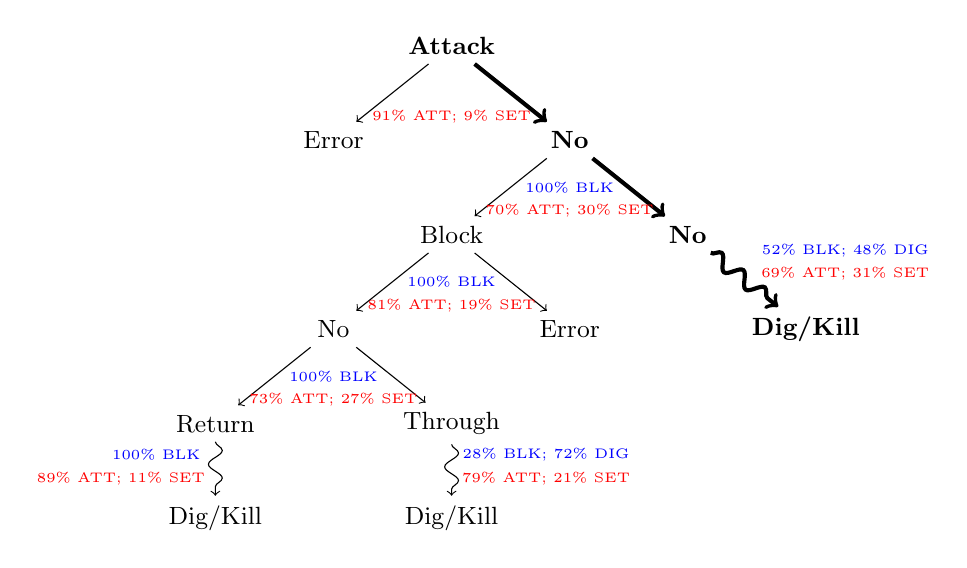
\begin{tikzpicture}
    \node (Attack) at (0, 0) {\small\bf Attack};
    \node (Attack Error) at (-1.5, -1.2) {\small Error};
    \node (Attack No Error) at (1.5, -1.2) {\small\bf No};
    \node (Block) at (0, -2.4) {\small Block};
    \node (No Block) at (3, -2.4) {\small\bf No};
    \node (Block No Error) at (-1.5, -3.6) {\small No};
    \node (Block Error) at (1.5, -3.6) {\small Error};
    \node (Return) at (-3, -4.8) {\small Return};
    \node (Through) at (0, -4.8) {\small Through};
    \node (No Block Dig/Kill) at (4.5, -3.6) {\small\bf Dig/Kill};
    \node (Return Dig/Kill) at (-3, -6) {\small Dig/Kill};
    \node (Through Dig/Kill) at (0, -6) {\small Dig/Kill};
    \draw[->] (Attack) -- (Attack Error);
    \draw[->, line width = 1.5pt] (Attack) -- (Attack No Error);
    \draw[->] (Attack No Error) -- (Block);
    \draw[->, line width = 1.5pt] (Attack No Error) -- (No Block);
    \draw[->] (Block) -- (Block No Error);
    \draw[->] (Block) -- (Block Error);
    \draw[->] (Block No Error) -- (Return);
    \draw[->] (Block No Error) -- (Through);
    \draw[->, line width = 1.5pt, decorate, decoration = snake] (No Block) -- (No Block Dig/Kill);
    \draw[->, decorate, decoration = snake] (Return) -- (Return Dig/Kill);
    \draw[->, decorate, decoration = snake] (Through) -- (Through Dig/Kill);
    \node at (0, -0.9) {\tiny \color{red} 91\% ATT; 9\% SET};
    \node at (1.5, -1.8) {\tiny \color{blue} 100\% BLK};
    \node at (1.5, -2.1) {\tiny \color{red} 70\% ATT; 30\% SET};
    \node at (0, -3) {\tiny \color{blue} 100\% BLK};
    \node at (0, -3.3) {\tiny \color{red} 81\% ATT; 19\% SET};
    \node at (-1.5, -4.2) {\tiny \color{blue} 100\% BLK};
    \node at (-1.5, -4.5) {\tiny \color{red} 73\% ATT; 27\% SET};
    \node at (1.2, -5.2) {\tiny \color{blue} 28\% BLK; 72\% DIG};
    \node at (1.2, -5.5) {\tiny \color{red} 79\% ATT; 21\% SET};
    \node at (-3.75, -5.2) {\tiny \color{blue} 100\% BLK};
    \node at (-4.2, -5.5) {\tiny \color{red} 89\% ATT; 11\% SET};
    \node at (5, -2.6) {\tiny \color{blue} 52\% BLK; 48\% DIG};
    \node at (5, -2.9) {\tiny \color{red} 69\% ATT; 31\% SET};
  \end{tikzpicture}
\end{frame}

\begin{frame}{{\it Example:} First Attack of 2022 National Championship}
  \begin{center}
    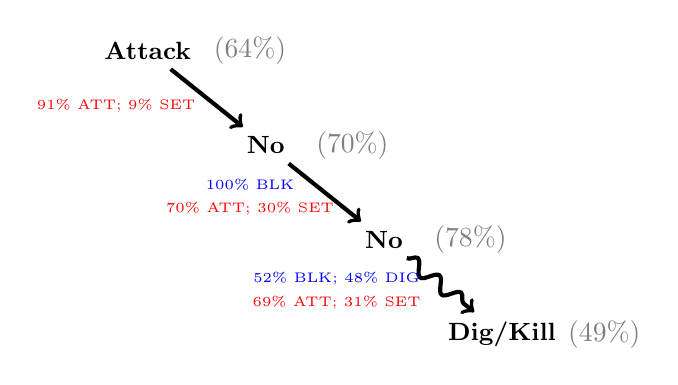
\begin{tikzpicture}
      \node (Attack) at (0, 0) {\small\bf Attack};
      \node at (1.3, 0) {\color{gray} (64\%)};
      \node (Attack No Error) at (1.5, -1.2) {\small\bf No};
      \node at (2.6, -1.2) {\color{gray}(70\%)};
      \node (No Block) at (3, -2.4) {\small\bf No};
      \node at (4.1, -2.4) {\color{gray}(78\%)};
      \node (No Block Dig/Kill) at (4.5, -3.6) {\small\bf Dig/Kill};
      \node at (5.8, -3.6) {\color{gray}(49\%)};
      \draw[->, line width = 1.5pt] (Attack) -- (Attack No Error);
      \draw[->, line width = 1.5pt] (Attack No Error) -- (No Block);
      \draw[->, line width = 1.5pt, decorate, decoration = snake] (No Block) -- (No Block Dig/Kill);
      \node at (-0.4, -0.7) {\tiny \color{red} 91\% ATT; 9\% SET};
      \node at (1.3, -1.7) {\tiny \color{blue} 100\% BLK};
      \node at (1.3, -2.0) {\tiny \color{red} 70\% ATT; 30\% SET};
      \node at (2.4, -2.9) {\tiny \color{blue} 52\% BLK; 48\% DIG};
      \node at (2.4, -3.2) {\tiny \color{red} 69\% ATT; 31\% SET};
    \end{tikzpicture}\\
    ~\\
    \small
    \begin{tabular}{c|ccc|c|c}
      \color{gray} TOT  & \color{gray}+6\% & \color{gray} +8\%  & \color{gray} --29\% & \color{gray} --15\% & \color{gray} Standard Stats\\
      \hline
      \color{red} ATT   & \color{red} +5\% & \color{red}  +6\%  & \color{red} --20\%  & \color{red}  --9\%  & \color{red} 1 attempt, 0 kills, 0 errors\\
      \color{red} SET   & \color{red} +1\% & \color{red}  +2\%  & \color{red}  --9\%  & \color{red}  --6\%  & \color{red} 0 assists\\
      \hline
      \color{blue} BLK  & \color{blue} --- & \color{blue} --8\% & \color{blue}  +15\% & \color{blue}   +7\% & \color{blue} ---\\
      \color{blue} DIG  & \color{blue} --- & \color{blue} ---   & \color{blue}  +14\% & \color{blue}  +14\% & \color{blue} 1 opportunity, 1 dig\\
    \end{tabular}
  \end{center}
  {\bf Caution:} Blocker/digger assignment is a work in progress
\end{frame}

\begin{frame}{Distribution of Points Gained per Opportunity}
  \includegraphics[width = \textwidth]{images/points_gained_per_opportunity.pdf}
\end{frame}

\begin{frame}{Standard vs. Advanced Metrics: Back Row Defense}
  \begin{columns}
    \begin{column}{0.59\textwidth}
      \includegraphics[width = \textwidth]{images/dig_comparison.pdf}
    \end{column}
    \begin{column}{0.41\textwidth}
      {\bf Player A:}\\
      72\% digs per opportunity\\
      +3.6\% PG per opportunity\\
      {
        \color{white}
        No block touch: 85\%\\
        Perfect dig rate: 48\%\\
      }
      ~\\
      {\bf Player B:}\\
      72\% digs per opportunity\\
      +1.2\% PG per opportunity\\
      {
        \color{white}
        No block touch: 66\%\\
        Perfect dig rate: 36\%\\
      }
    \end{column}
  \end{columns}
  ~\\
  {\bf Caution:} Dig evaluation codes are biased against setters by design
\end{frame}

\begin{frame}[noframenumbering]{Standard vs. Advanced Metrics: Back Row Defense}
  \begin{columns}
    \begin{column}{0.59\textwidth}
      \includegraphics[width = \textwidth]{images/dig_comparison.pdf}
    \end{column}
    \begin{column}{0.41\textwidth}
      {\bf Player A:}\\
      72\% digs per opportunity\\
      +3.6\% PG per opportunity\\
      {
        \color{ricerichblue}
        No block touch: 85\%\\
        Perfect dig rate: 48\%\\
      }
      ~\\
      {\bf Player B:}\\
      72\% digs per opportunity\\
      +1.2\% PG per opportunity\\
      {
        \color{ricerichblue}
        No block touch: 66\%\\
        Perfect dig rate: 36\%\\
      }
    \end{column}
  \end{columns}
  ~\\
  {\bf Caution:} Dig evaluation codes are biased against setters by design
\end{frame}

\begin{frame}
  \centering
  {\color{riceblue} \bf Act 3: Adjusting for Strength of Schedule}\\
  {\color{ricegray} \it Technique: Linear Mixed-Effect Models}
\end{frame}

\begin{frame}{Server vs. Receiver}
  Exp. Points Gained = $\beta_{\mbox{\scriptsize Server}}$ + $\delta_{\mbox{\scriptsize Receiver}}$ \hfill (good)\\
  ~\\
  \pause
  Exp. Points Gained = $(\beta_{\mbox{\scriptsize Team}} + \beta_{\mbox{\scriptsize Server}})$ + \hfill (better)\\
  \hspace{3.7cm} $(\delta_{\mbox{\scriptsize Team}} + \delta_{\mbox{\scriptsize Receiver}})$\\
  ~\\
  \pause
  Exp. Points Gained = $(\beta_{\mbox{\scriptsize Conf}} + \beta_{\mbox{\scriptsize Team}} + \beta_{\mbox{\scriptsize Server}})$ + \hfill(best)\\
  \hspace{3.7cm} $(\delta_{\mbox{\scriptsize Conf}} + \delta_{\mbox{\scriptsize Team}} + \delta_{\mbox{\scriptsize Receiver}})$\\
  ~\\
  \pause
  \begin{itemize}
    \item Fit random-effects model using lme4 package in R
  \end{itemize}
  ~\\
  Server:\\
  Adj. Points Gained $\approx$ Points Gained -- $(\hat\delta_{\mbox{\scriptsize Conf}} + \hat\delta_{\mbox{\scriptsize Team}} + \hat\delta_{\mbox{\scriptsize Receiver}})$
  \begin{itemize}
    \item Requires a de-biasing step
    \item Some generalization required for extension to other skills
  \end{itemize}
\end{frame}

\begin{frame}{Results: Top 10 Conferences (all skills)}
  \centering
  \begin{tabular}{c|c}
    Conference      & Avg SoS\\
    \hline
    Big Ten         & +0.23\\
    Pac-12          & +0.23\\
    SEC             & +0.21\\
    Big 12          & +0.20\\
    ACC             & +0.15\\
    West Coast      & +0.09\\
    American        & +0.04\\
    Big West        & +0.04\\
    Mountain West   & +0.02\\
    Mid-American    & +0.01
  \end{tabular}\\
  \vspace{1cm}
  \footnotesize SoS units: points gained per set
\end{frame}

\begin{frame}{{\it Example:} Conference Comparison (all skills)}
  \includegraphics[width = \textwidth]{images/conference_comparison.pdf}
  \begin{itemize}
    \item Separation between conferences is evident
    \item One elite player from the Summit League still stands out
  \end{itemize}
  {\bf Caution:} Additive assumption is not literally true in real life
\end{frame}

\begin{frame}{{\it Example:} Teammate Comparison (outside hitters)}
  \begin{columns}
    \begin{column}{0.5\columnwidth}
      \includegraphics[width = \textwidth]{images/teammate_comparison.pdf}
    \end{column}
    \begin{column}{0.5\columnwidth}
      \begin{itemize}
        \item Player A average SOS: +1.4\% (PG per attack)\\
        ~\\
        \item Player B average SOS: --0.1\% (PG per attack)
      \end{itemize}
    \end{column}
  \end{columns}
  \begin{center}
    Toughest SoS: Player A vs. Nebraska, +13.0\%\\
    Kaitlyn Hord blocking, Lexi Rodriguez digging
  \end{center}
  {\bf Caution:} SoS depends on which zone the attacker hits
\end{frame}

\begin{frame}
  \centering
  \color{riceblue} \bf (Act 4: Discussion)\\
\end{frame}

\begin{frame}{Question: Where does Logan Eggleston rank?}
  \pause
  \centering
  \includegraphics[width = 0.6\textwidth]{images/avca_all_americans_adj.pdf}\\
  \includegraphics[width = \textwidth]{images/top_ten_players.png}
\end{frame}

\begin{frame}{Application: Defensive Specialist Strategy}
  \begin{itemize}
    \item 63\% of teams replace at least one OH with a DS in back row
  \end{itemize}
  \vspace{2mm}
  \begin{columns}
    \begin{column}{0.5\textwidth}
      \centering
      \includegraphics[width = \textwidth]{images/oh_comparison.pdf}
    \end{column}
    \begin{column}{0.5\textwidth}
      \small
      \underline{Reception PG per opportunity}\\
      ~\\
      \color{ricerichblue} All-Around OH: $+1.1\%$\\
      ~\\
      \color{ricegray} Front-Only OH: $-1.4\%$\\
      ~\\
      \color{white} Defensive Specialist: $+0.9\%$\\
      ~\\
      \color{white} Substitutable Opportunities:\\
      0.1 opportunities per point
    \end{column}
  \end{columns}
  \vspace{4mm}
  \begin{itemize}
    \color{white}
    \item[\color{white}] {\it Example:} Point win probability $50\% \rightarrow 50.2\%$
    \begin{itemize}
      \color{white}
      \item[\color{white}] Match win probability $50\% \rightarrow 52\%$
    \end{itemize}
  \end{itemize}
  \vspace{3mm}
  \centering
  \footnotesize
  \color{white}
  Pythagorean formula for volleyball: $p^{10} / (p^{10} + (1-p)^{10})$
\end{frame}

\begin{frame}[noframenumbering]{Application: Defensive Specialist Strategy}
  \begin{itemize}
    \item 63\% of teams replace at least one OH with a DS in back row
  \end{itemize}
  \vspace{2mm}
  \begin{columns}
    \begin{column}{0.5\textwidth}
      \centering
      \includegraphics[width = \textwidth]{images/oh_comparison_with_ds.pdf}
    \end{column}
    \begin{column}{0.5\textwidth}
      \small
      \underline{Reception PG per opportunity}\\
      ~\\
      \color{ricerichblue} All-Around OH: $+1.1\%$\\
      ~\\
      \color{ricegray} Front-Only OH: $-1.4\%$\\
      ~\\
      \color{riceblue} Defensive Specialist: $+0.9\%$\\
      ~\\
      \color{black} Substitutable Opportunities:\\
      0.1 opportunities per point
    \end{column}
  \end{columns}
  \vspace{4mm}
  \pause
  \begin{itemize}
    \item {\it Example:} Point win probability $50\% \rightarrow 50.2\%$
    \begin{itemize}
      \item Match win probability $50\% \rightarrow 52\%$
    \end{itemize}
  \end{itemize}
  \vspace{3mm}
  \centering
  \footnotesize
  Pythagorean formula for volleyball: $p^{10} / (p^{10} + (1-p)^{10})$
\end{frame}

\begin{frame}{Limitations and Next Steps}
  \begin{itemize}
    \item Improve blocker and digger assignments
    \item Correct bias for digs made by setter
    \item Reward good decision-making in strength of schedule
    \item Account for whether setter is back row or front row
    \item Leverage (X, Y) coordinate information
  \end{itemize}
\end{frame}

\begin{frame}
  \centering
  \LARGE
  Thank You!
\end{frame}

\end{document}